\chapter{Introduction} % 1 page max
\label{ch:Introduction}


\section{Contexte et objectif}
\label{sec:Contexte}

L'\textbf{informatique quantique} est un domaine en plein essor. Cette technologie permettant de manipuler des qubits à la place des bits qui sont à la base de l'informatique actuelle, ouvrent la voie à des algorithmes plus performants que les algorithmes classiques. Les machines quantiques exécutant ces algorithmes étant encore en développement et d'un coût important, il existe un besoin d'outils de simulation et de vérification d'algorithmes quantiques par des machines classiques. L'objectif de ce projet est de proposer un modèle de la structure de données des diagrammes de décision quantiques additifs abstraits, en s'appuyant sur les travaux existants, et de les simuler pour en étudier les performances.


\section{État de l’art}
\label{sec:Etat}


\subsubsection*{Informatique quantique}

Le premier postulat de la physique quantique, le \textbf{principe de superposition}, énonce que l'espace des états d'un système quantique est un espace de Hilbert. Par conséquent, si un \textit{bit} ne peut classiquement être que dans un état $\ket 0$ ou $\ket 1$, son homologue quantique, le \textbf{qubit}, peut être dans une superposition de ces deux états.
$$\ket \psi = \alpha \ket 0 + \beta \ket 1$$

\noindent où $\alpha, \beta$ sont des coefficients complexes. Le second postulat, le \textit{principe de mesure}, stipule que lorsqu'un qubit est mesuré, il est projeté sur un des états de base $\ket 0$ ou $\ket 1$ avec une probabilité $|\alpha|^2$ ou $|\beta|^2$ respectivement.

Les états à $n$ qubits peuvent être représentés par des \textbf{vecteurs} de dimension $2^n$, les états de l'ensemble constitué de deux systèmes étant ceux obtenus par produit tensoriel (\textit{produit de Kronecker}) d'un état du premier système et d'un état du second. C'est ce nombre exponentiel de paramètres complexes pour un état à plusieurs qubits qui rend l'étude classique d'algorithmes quantiques difficile, puisque les états prennent une taille exponentiellement grande en mémoire.

\vspace{1em}

Comme en informatique classique, les opérations élémentaires sur la mémoire sont réalisées en informatique quantique par des \textbf{portes}. D'un point de vue mathématique, une porte opérant sur $n$ qubits est couramment représentée par une matrice de taille $2^n \times 2^n$. Appliquer une porte $M$ à un ensemble de qubits $v$ revient alors à multiplier le vecteur d'état par la matrice de la porte.

L'application en parallèle de plusieurs portes sur plusieurs qubits est représentée par le \textbf{produit tensoriel} (produit de Kronecker) des matrices de portes. On note toutefois que l'application de cette manière de portes sur des qubits se fait en un temps exponentiel en fonction du nombre de qubits, ce qui rend l'utilisation naïve d'algorithmes quantiques sur des machines classiques inefficace.

L'application de portes à des qubits est fréquemment représentée sous forme de \textbf{circuits quantiques}, où les qubits sont représentés par des lignes et les portes par des boîtes.

\begin{figure}
  \centering
  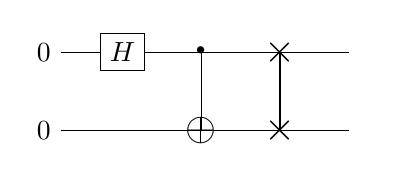
\begin{tikzpicture}
    \node (end1) at (4, 0) {};
    \node (end2) at (4, -1) {};
    \node (q1) at (0, 0) {$\ket 0$};
    \node (q2) at (0, -1) {$\ket 0$};

    \node [draw] (h1) at (1, 0) {$H$};
    \draw (q1) -- (h1);
    \draw (h1) -- (end1);
    \draw (q2) -- (end2);
    \node (cx) at (2, -1) {\Large $\oplus$};
    \node (cx2) at (2, 0) {\Huge $\cdot$};
    \node (s1) at (3, 0) {\Large $\times$};
    \node (s2) at (3, -1) {\Large $\times$};

    \draw (s1.center) -- (s2.center);
    \draw (cx2.center) -- (cx.center);
  \end{tikzpicture}
  \caption{Circuit à 2 qubits avec les portes $H$, $CX$ et $S$}
\end{figure}

N'importe quelle matrice \textit{unitaire} et \textit{réversible} peut être utilisée comme porte quantique. Parmi les portes les plus courantes, on compte la porte de Hadamard ($H$), la porte « non » ($X$), la porte « non contrôlée » ($CX$), ou la porte d'échange ($S$ pour \textit{swap}). Ces portes sont avec d'autres utilisées pour réaliser des algorithmes quantiques, comme l'algorithme de Deutsch-Josza \cite{DJ_1992}, l'algorithme de Grover \cite{Grover_1996}, ou encore celui de Shor \cite{Shor_1997}.

\vspace{1em}

Afin de proposer un langage unifié permettant de développer des algorithmes quantiques à partir de portes pouvant être interprété sur n'importe quel matériel, IBM a publié en 2017 le langage de programmation \textbf{Open QASM}. \cite{QASM_2017} On y définit des qubits sur lesquels on applique des portes, et on peut ensuite simuler ou exécuter le programme sur un ordinateur quantique comme sur un ordinateur classique. Le circuit précédent peut par exemple être représenté par le programme \ref{lst:QASM}. :

\begin{figure}[thp]
  \renewcommand{\figurename}{Programme}
  \centering
\begin{tabular}{c}
\begin{lstlisting}
  qubit a;
  qubit b;
  h a;
  cx a b;
  s a b;
\end{lstlisting}
\end{tabular}
\caption{Exemple de code Open QASM}
\label{lst:QASM}
\end{figure}

\subsubsection*{Diagrammes de décision}

La structure de \textbf{diagramme de décision} est une structure de données développée à partir des années 1970. Elle est depuis devenue largement utilisée en informatique, notamment pour rendre plus compacte la représentation de \textbf{fonctions binaires} \cite{Minato_1996}.

Prenons par exemple la fonction binaire $f(x_1, x_2, x_3) = x_1 \lor (x_2 \land x_3)$. La représentation d'une telle fonction se fait dans le cas général à l'aide d'une \textit{table de vérité}, donc dans une taille grandissant exponentiellement par rapport au nombre de variables binaires considéré. On peut utiliser une représentation plus compacte en utilisant un diagramme de décision, comme le montre la \autoref{fig:ExempleDD}, où les fils gauches sont signalés par des flèches pointillées et les fils droits sont signalés par des flèches continues.

\begin{figure}
  \renewcommand{\arraystretch}{0.8}% Tighter
  \begin{tabular}{c|c|c|c}
    $x_1$ & $x_2$ & $x_3$ & $f(x_1, x_2)$ \\
    \hline
    0 & 0 & 0 & 0 \\
    0 & 0 & 1 & 0 \\
    0 & 1 & 0 & 0 \\
    0 & 1 & 1 & 1 \\
    1 & 0 & 0 & 1 \\
    1 & 0 & 1 & 1 \\
    1 & 1 & 0 & 1 \\
    1 & 1 & 1 & 1
  \end{tabular}
  \hfill{}
  % https://tikzcd.yichuanshen.de/#N4Igdg9gJgpgziAXAbVABwnAlgFyxMJZAJgBoAGAXVJADcBDAGwFcYkQAPAfQEYACADoDGEAE58AFN2KDh9MFD7cAzAEoQAX1LpMufIRTLSy6nSat2PTdpAZseAkXIVTDFm0QgpvdVp339J1IeV3MPL2lfGzs9RxRnYlD3dm81a39Yg2QeYySLT3J0210HLJyQmjd8zi4ZIUZ5RRUimNKiMkTKsPZmjVMYKABzeCJQADNRCABbJGcQHAgkADYaRiwwcKh6OAALAaKJ6dmaBaQckAAjGAUkZTmq8O5+AF4+Kz8QQ5nEFfnFxAArKt1pttnsoCAuslPNJnoVVvQrowAAolQKeURYQY7HAHSbfX6nRAAdih1Vh7xsXyQpL+SCBIDWG3YW12+zJjy4yj4r0KH2pJJO-3ODx6XOe70oGiAA
  \begin{tikzcd}[column sep=tiny]
    (x_1) &                                                                & x_1 \lor (x_2 \land x_3) \arrow[ld, dashed] \arrow[rddd, "x_1 = 1", bend left] &   \\
    (x_2) & x_2 \land x_3 \arrow[dd, "x_2=0"', dashed] \arrow[rd, "x_2=1"] &                                                                                &   \\
    (x_3) &                                                                & x_3 \arrow[ld, "x_3 = 0", dashed] \arrow[rd, "x_3=1"]                          &   \\
          & 0                                                              &                                                                                & 1
    \end{tikzcd}
    \hfill{}
  % https://tikzcd.yichuanshen.de/#N4Igdg9gJgpgziAXAbVABwnAlgFyxMJZARgBoAGAXVJADcBDAGwFcYkQQBfU9TXfQigBMpAMzU6TVu2JceIDNjwEi5MRIYs2iEOTm8lA1aWIap2jtwP8VKMkLNb2XCTCgBzeEVAAzAE4QALZIaiA4EEiiNIxYYBZQ9HAAFm76IP5BITThSGQgAEYwYFCR5FbpAcGIUWERiCIgMXHsCcmp0fSFjAAKfMqCIH5Y7kk4aRlVNTmIACzlE0gz2XUNTfGJKSXzlYvLuZyUnEA
  \begin{tikzcd}[column sep=huge, row sep=large]
    & {} \arrow[ld, dashed] \arrow[rddd, bend left] &   \\
  {} \arrow[dd, dashed] \arrow[rd] &                                               &   \\
    & {} \arrow[ld, dashed] \arrow[rd]              &   \\
  0                                &                                               & 1
  \end{tikzcd}

  \caption{(a) Table de vérité (b) Diagramme de décision (c) Diagramme de décision sans labels}
  \label{fig:ExempleDD}
\end{figure}

Les diagrammes de décision prennent avantage de la \textbf{structure} interne de la donnée (ici, une fonction booléenne). On note d'une part que les labels ne sont pas nécessaires pour reconstituer les valeurs prises par la fonction.
D'autre part, dans le pire des cas, c'est-à-dire celui où la fonction ne possède aucune structure permettant une réduction, la taille du diagramme de décision (son nombre de branches) vaut $2^{n+1} - 2$ ce qui comme le nombre de valeurs $2^n$ à stocker dans une table de vérité, est \textbf{exponentiel} en $n$. Dans le pire cas, les diagrammes de décision ne permettent pas d'amélioration, mais ne sont pas non plus asymptotiquement pire que les tables de vérité.


\subsubsection*{Interprétation abstraite}

L'interprétation abstraite est une méthode générale consistant à traiter des propriétés de programmes informatiques en les abstrayant. Elle a été introduite par Patrick et Radhia Cousot en 1977 \cite{CousotCousot77-1}. Elle peut aussi être utilisée pour résoudre des problèmes ou calculer plus rapidement.

Étudions le problème suivant : on cherche à déterminer le signe de  l'expression $-12 \times 7 - 13$. On pourrait calculer le résultat de cette expression, mais on peut aussi remarquer que $-12$ et $-13$ sont négatifs et que 7 est positif, d'où $-12 \times 7$ négatif, ainsi l'expression est négative. Plus formellement, on est parti des \textbf{éléments concrets} que sont $-12$, 7 et $-13$ et on les a remplacés par les \textbf{éléments abstraits} « positif » $\oplus$ et « négatif » $\ominus$, sur lesquels on définit les opérations de somme et de produit selon les règles bien connues.

Il existe de nombreux cas d'utilisation de l'interprétation abstraite \cite{Rosendahl_1995}, pour la compilation de programmes par exemple. Nous l'utiliserons dans ce projet pour simplifier les diagrammes de décision quantiques quitte à perdre une partie de l'information qu'ils contiennent. C'est aussi le cas pour l'exemple précédent : abstraire les éléments par leur signe ne permet pas toujours de déterminer le signe de l'expression.


\section{Contribution}
\label{sec:Contribution}

Les différents concepts présentés dans l'état de l'art permettent tous d'améliorer la vitesse de calcul ou la taille en mémoire d'une donnée. Il s'agit donc de \textbf{combiner ces concepts} dans ce projet, en ajoutant une dimension supplémentaire, l'additivité : le fait pour un diagramme d'avoir plusieurs fils droits (respectivement gauches), l'interprétation étant que le « fils droit effectif » est la somme des fils droits (respectivement gauches) du diagramme.
L'objectif du projet était donc de proposer un modèle de diagrammes de décision quantiques abstraits et additifs, et de les simuler pour en étudier les performances en comparaison d'autres modèles.

De manière préliminaire, une étude des intervalles complexes polaires a été réalisée, ce qui n'avait pas été fait jusqu'à présent.
Un \textbf{modèle} mathématique de la structure de données et de méthodes de réduction ont été formalisés, et des algorithmes de réduction ont été développés pour simplifier ces diagrammes.
De plus, une des méthodes d'application de portes quantiques aux diagrammes ont été formalisées.
Une \textbf{implémentation} de ces algorithmes a été réalisée, sans se baser sur des bibliothèques existantes (mis à part pour les tests unitaires).

\section{Structure du rapport}
\label{sec:Structure}

Le \autoref{ch:Modele} présente le modèle théorique de diagrammes de décision quantiques qui a été développé, y compris les algorithmes de réduction et d'application de portes qui accompagnent celui-ci. Ensuite, le \autoref{ch:Implementation} discute de l'implémentation réalisée. Finalement, une courte conclusion est présentée dans le \autoref{ch:Conclusion}.

Un document théorique plus complet que ce rapport destiné à être publié et rédigé en anglais, est disponible en ligne. D'éventuels points théoriques succinctement présentés dans ce rapport et ou théorèmes dont la preuve n'est pas spécifiée sont détaillés dans ce document. \cite{Leroy_2025} De plus, une documentation technique du code est disponible en ligne. \cite{Leroy_doc}
